\begin{figure}[H]
\centering
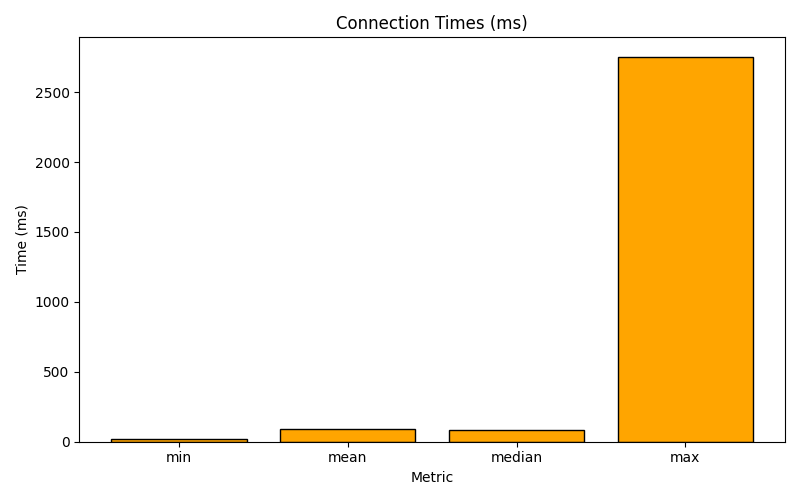
\includegraphics[width=0.85\textwidth]{ab_connection_times}
\caption*{\small{\textbf{Εικόνα 4.1} Χρονικές καθυστερήσεις συνδέσεων (ms) από με Apache Bench}}
\end{figure}

\begin{figure}[H]
\centering
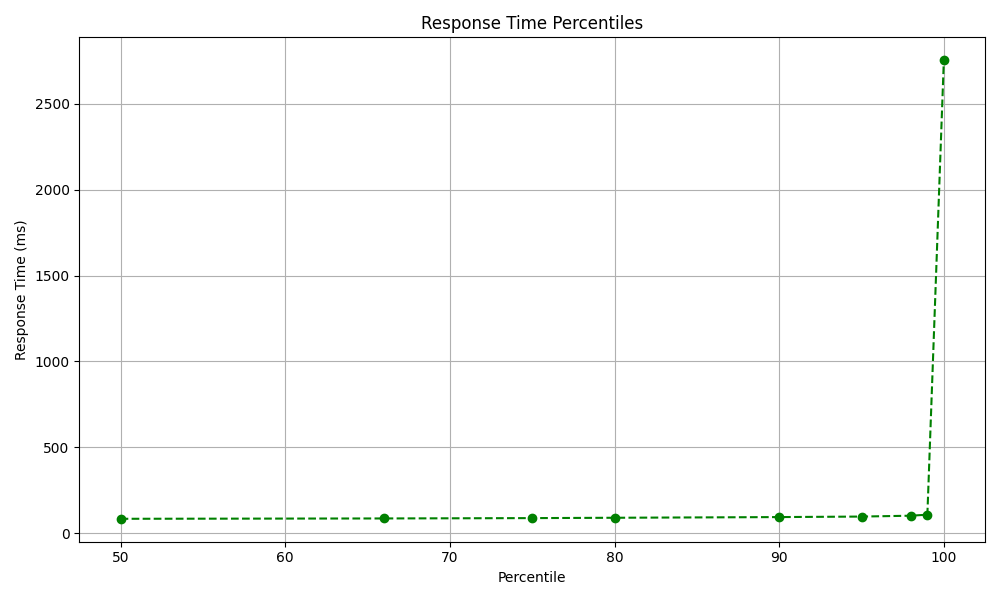
\includegraphics[width=0.85\textwidth]{ab_percentile}
\caption*{\small{\textbf{Εικόνα 4.2} Χρονικές καθυστερήσεις συνδέσεων (ms) από με Apache Bench (percentile)}}
\end{figure}

\begin{figure}[H]
\centering
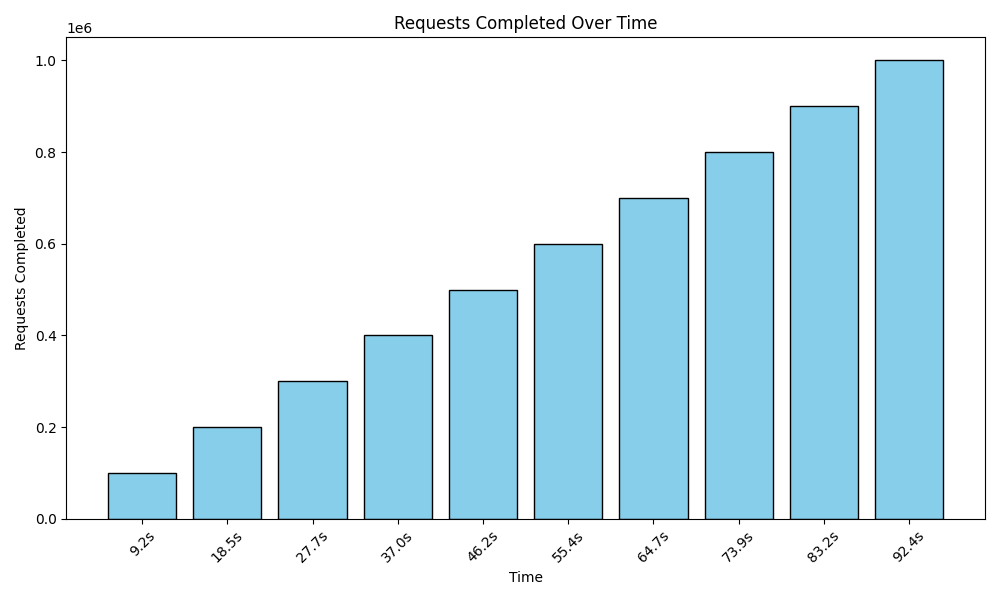
\includegraphics[width=0.85\textwidth]{ab_requests_over_time}
\caption*{\small{\textbf{Εικόνα 4.3} Ολοκληρωμένα αιτήματα με την πάροδο του χρόνου}}
\end{figure}

\begin{figure}[H]
\centering
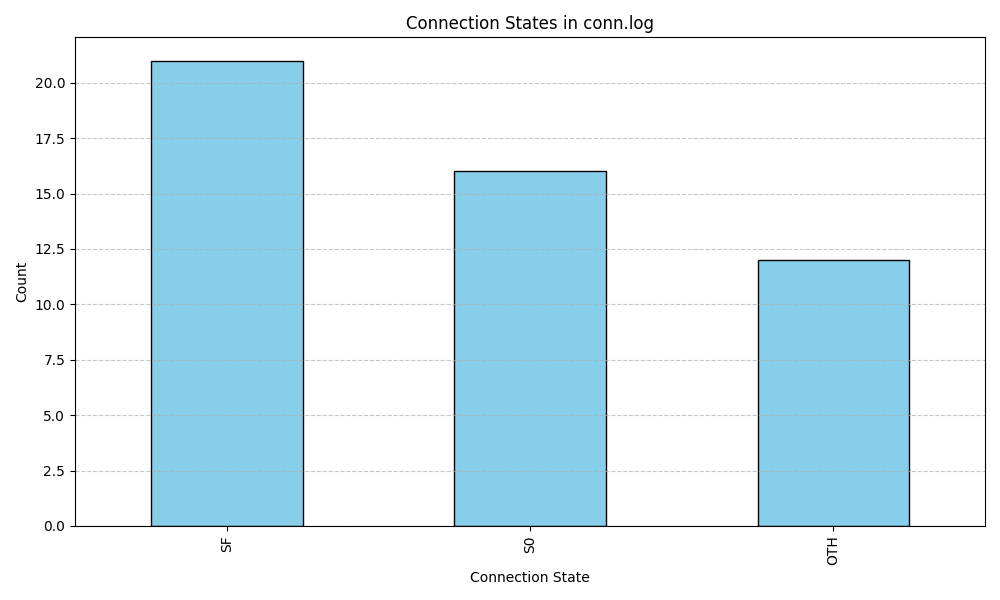
\includegraphics[width=0.85\textwidth]{connection_states}
\caption*{\small{\textbf{Εικόνα 4.4} Καταστάσεις σύνδεσης στο αρχείο conn.log: SF (Επιτυχής Σύνδεση), S0 (Προσπάθεια Σύνδεσης, Χωρίς Απάντηση), OTH (Άλλη Κατάσταση)}}
\end{figure}

Προκειμένου να οπτικοποιηθούν τα alerts που έχει παράγει το Zeek, χρησιμοποιήθηκαν τα logs που προέκυψαν. Στη συνέχεια, χρησιμοποιήθηκαν οι βιβλιοθήκες pandas και matplotlib. Επιπρόσθετα, χρησιμοποιώντας οδηγό από το \href{https://github.com/hackertarget/pcap-did-what/blob/master/zeek-docker/zeek-to-sqlite.py}{Github} μετατράπηκαν τα log files της \textbf{Zeek} σε μία \textbf{sqlite3} βάση δεδομένων όπου μετεπειτα φορτώθηκε σε ένα υπάρχον dashboard σε ένα self hosted Grafana instance.

\begin{figure}[H]
\centering
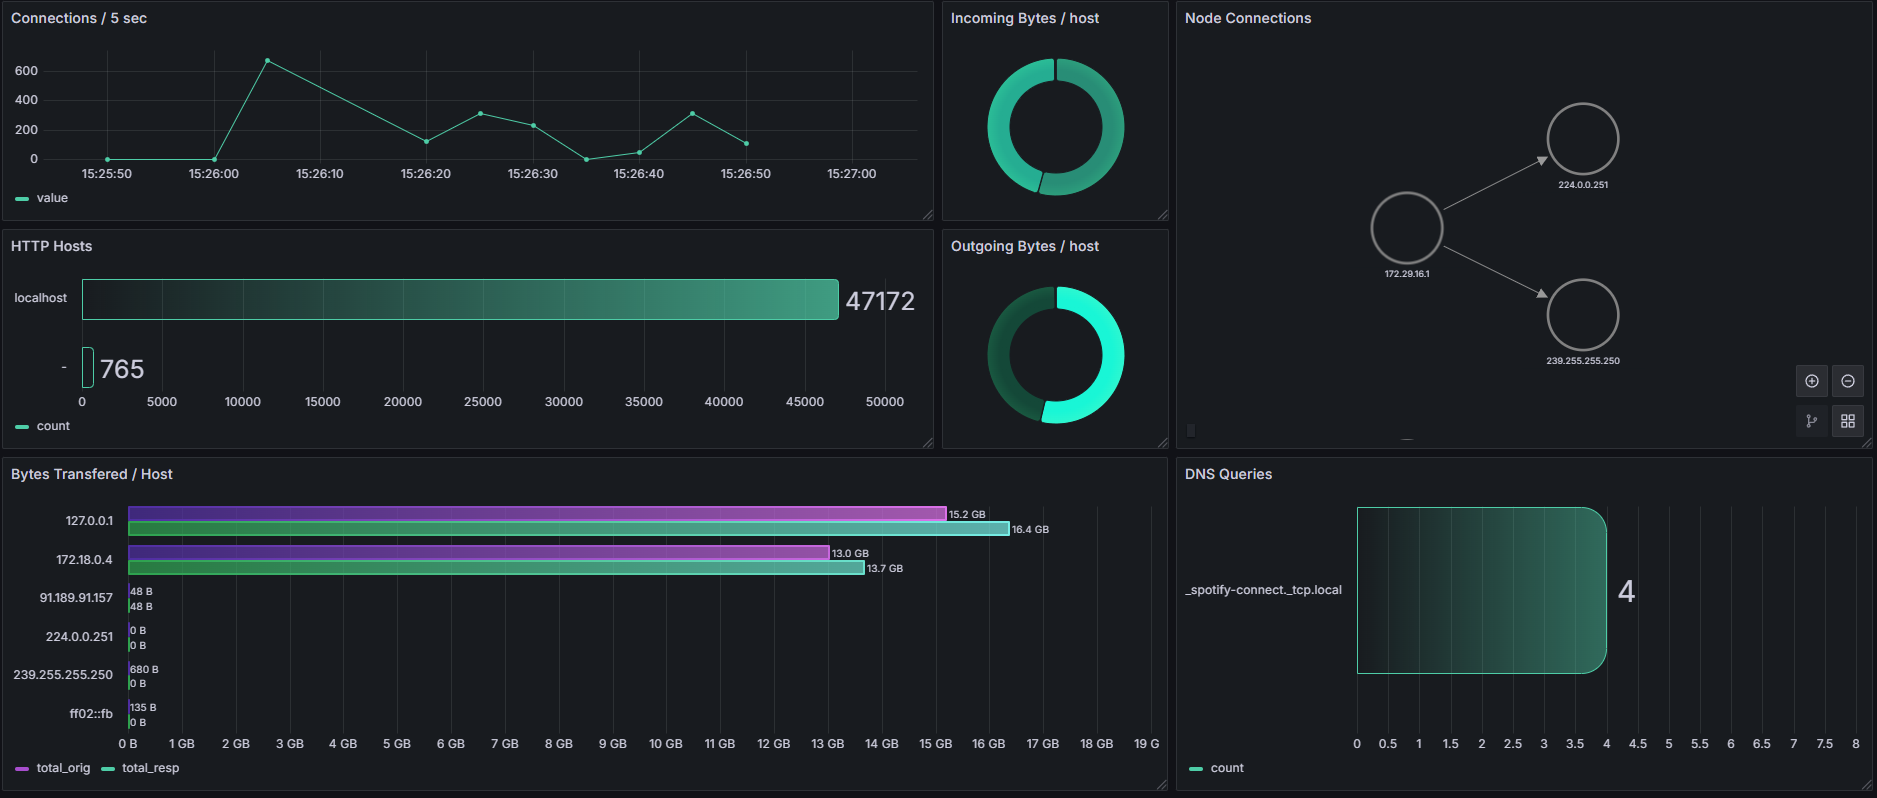
\includegraphics[width=0.85\textwidth]{graphana_og}
\caption*{\small{\textbf{Εικόνα 4.5} Το UI του \textbf{Grafana}}}
\end{figure}

\begin{figure}[H]
\centering
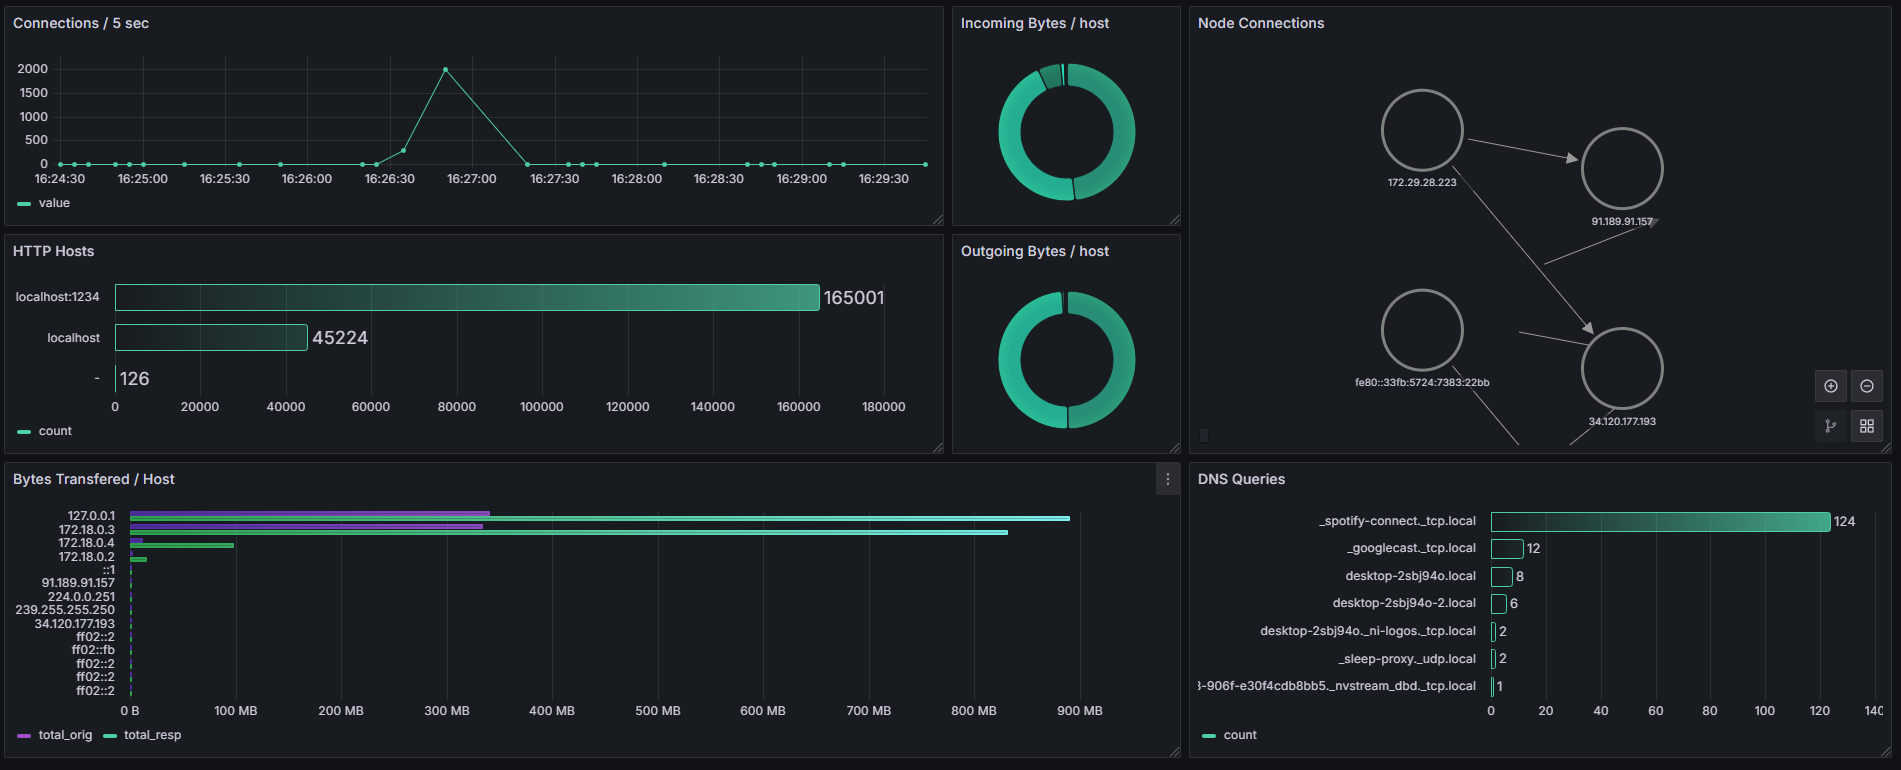
\includegraphics[width=0.85\textwidth]{graphana_1}
\caption*{\small{\textbf{Εικόνα 4.6} Το \textbf{Grafana} μετά από κάποια ώρα λειτουργίας }}
\end{figure}